\section{Conclusion}
To bring this back to where we started, we saw that individual stock returns exhibit positive skewness that can be phased by diversifying. This requires markets, and specifically public equity issuance, which requires the amelioration of moral hazard\textemdash something regulation can accomplish. The aggregate market is still risky (exhibits excess kurtosis), yet we do know that it is not well-described by a normal distribution. Besides heavy tails, aggregate market returns exhibit negative skewness, implying that negative events tend to go together.

Option prices reflect these heavy-tailed returns, though they did not always, reflecting another source of uncertainty: uncertainty in models. Models are important because judging the future purely by past events without understanding leaves us exposed to the chicken problem. We can be lured by a safe time series into thinking that nothing bad will happen; we can also be lured into believing a model representing safety is correct if we are not willing to consider alternatives. If our beliefs are confounded by recency bias, this will be difficult, and research shows that recent events, especially if they are noticeable like stock returns, do inform beliefs and survey responses. But a closer look shows that the entire lifetime of experience matters, paving the way for a memory-based model.

Yet the most remarkable finding may be what was truly unexpected: the extraordinary performance of the stock market over the last 100 years. While daily returns on the aggregate market are negatively skewed, the distribution of long-run returns is highly positively skewed. One dollar invested grows more than four-fold, even adjusting for inflation as shown in \autoref{fig:fig19} \citep{binsbergen2023united}. This is a remarkable success story that would have come entirely as a surprise back in the $1920s$. The idea that one might give a risky venture money and expect to be paid off is surprising, but it is regulation that controls, for example, the moral hazard problem, that makes this possible.

\begin{figure}[h]
    \centering
    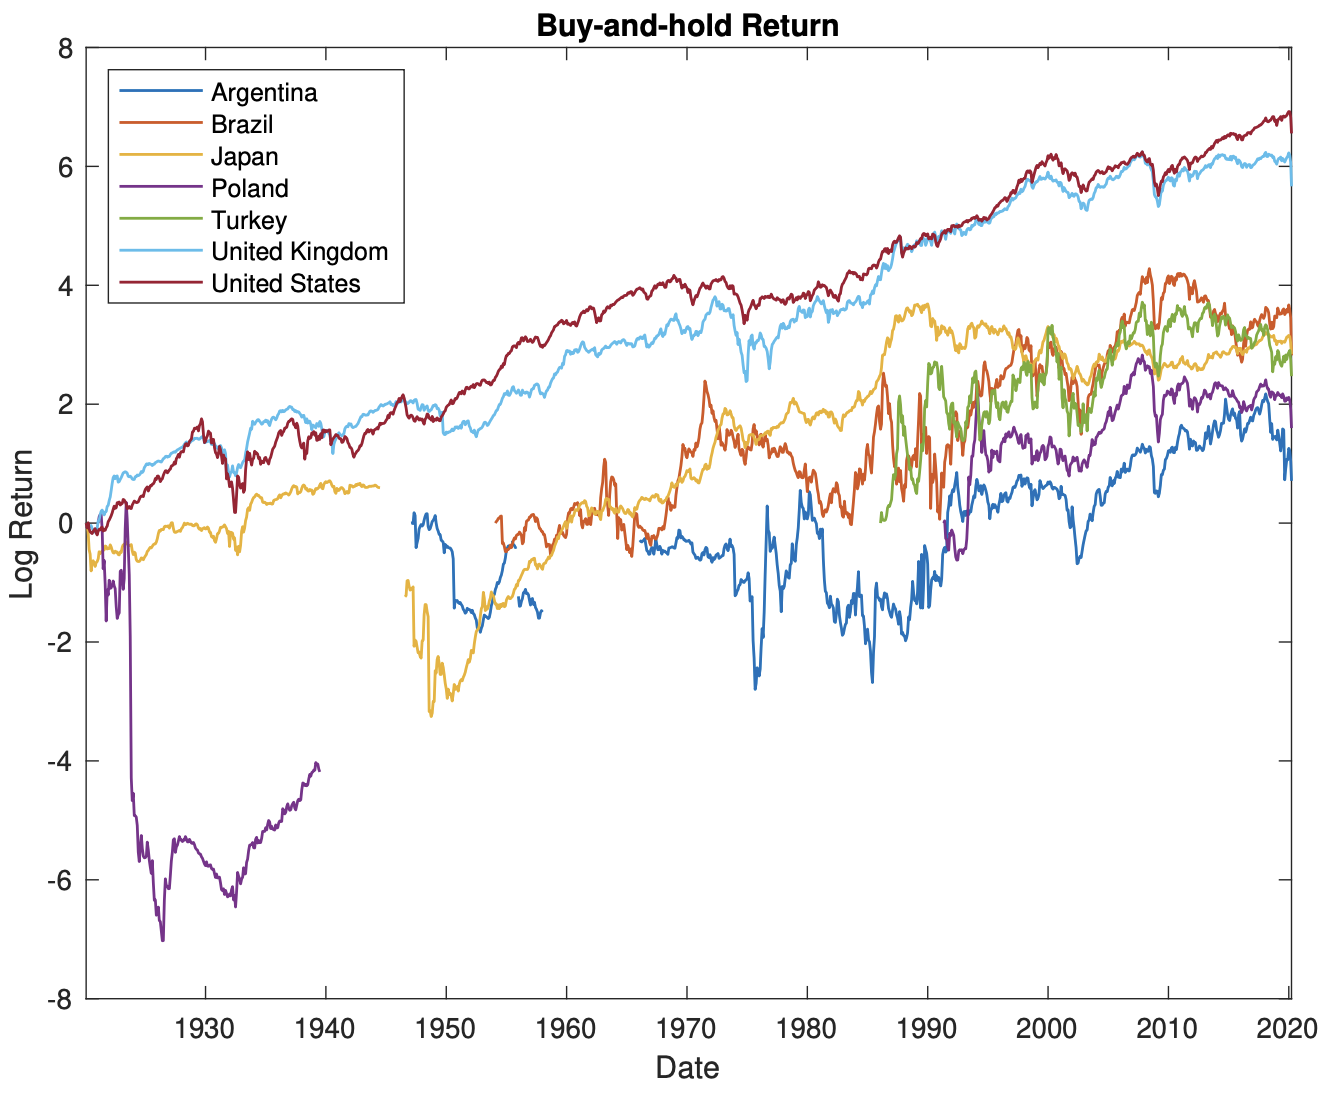
\includegraphics[width=0.75\textwidth]{fig19.png}
    \caption{Stock market returns \citep{binsbergen2023united}}
    \label{fig:fig19}
\end{figure}

Decades of research have failed to account for this based on standard methods of risk. Rather, it appears that this was a continuous surprise. It is a remarkable story, and an unexpected one, that reforms set up in the $1930s$ and $1940s$ would have worked so well in allowing capital to grow. In the long run, skewness in market returns is positive, not negative. The unexpected was this positive event, that a regulatory regime established in the $1930s$ and $1940s$ would work so surprisingly well. Understanding this tension between short-run tail risks and long-run positive surprises may be the most important lesson finance has to offer. 
